% !TEX program = pdflatex
\documentclass[letterpaper,12pt]{article}
\usepackage[spanish,mexico]{babel}
\usepackage[T1]{fontenc}
\usepackage{lmodern}
\usepackage{amsmath,amssymb}
\usepackage{graphicx,float,subcaption,xcolor,array,booktabs,tabularx,ragged2e}
\usepackage{tikz}
\usetikzlibrary{positioning,arrows.meta,calc,shapes.geometric}
\usepackage{listings}
\usepackage{pdflscape}
\usepackage[left=25mm,right=25mm,top=35mm,bottom=30mm,headheight=15pt]{geometry}
\usepackage{parskip,fancyhdr}
\usepackage{hyperref}

\graphicspath{{img/}{portada_img/}}
\newcommand{\materia}{Laboratorio de Organización y Arquitectura de Computadoras}
\newcommand{\pendiente}[1]{\fbox{\parbox[c][48mm][c]{0.88\linewidth}{\centering\textit{Espacio reservado para #1.}\\[2mm]\small Inserte aquí la evidencia cuando esté disponible.}}}
\pagestyle{fancy}
\fancyhf{}
\fancyhead[R]{\textsc{\materia}}
\fancyfoot[C]{\thepage}
\renewcommand{\headrulewidth}{0.8pt}
\hypersetup{colorlinks=true,linkcolor=blue,urlcolor=cyan}

\definecolor{codebg}{rgb}{0.96,0.96,0.96}
\definecolor{keyword}{rgb}{0.0,0.2,0.6}
\definecolor{comment}{rgb}{0.25,0.5,0.35}
\definecolor{codegray}{rgb}{0.5,0.5,0.5}
\lstdefinestyle{estiloVHDL}{
  language=VHDL,basicstyle=\ttfamily\scriptsize,
  backgroundcolor=\color{codebg},commentstyle=\color{comment}\itshape,
  keywordstyle=\color{keyword}\bfseries,numbers=left,
  numberstyle=\tiny\color{codegray},frame=single,breaklines=true,
  keepspaces=true,showstringspaces=false,tabsize=4,
  morekeywords={library,use,all,entity,is,port,in,out,architecture,of,begin,end,signal,constant,process,if,then,else,elsif,case,when,others,std_logic,std_logic_vector}
}

\begin{document}
\thispagestyle{empty} % Sin encabezado ni pie en la portada

% --- ENCABEZADO DE PORTADA (TABLA DE 3 COLUMNAS) ---
\begin{center}
    % La tabla usa 'm' para centrar verticalmente las imágenes y el texto
    \begin{tabular}{m{0.15\textwidth} m{0.60\textwidth} m{0.15\textwidth}}
        % Logo Izquierdo (UNAM)
        
\includegraphics[width=2cm]{portada_img/escudounam_negro.jpg} & 
        
        % Título Central
        \centering\Huge\textbf{Universidad Nacional Autónoma de México} &
        
        % Logo Derecho (Facultad)
        \raggedleft
\includegraphics[width=2cm]{portada_img/escudofi_negro.jpg}
    \end{tabular}
\end{center}

\vspace{0.3cm}

% --- INFORMACIÓN DEL REPORTE ---
\begin{center}
    {\LARGE \textbf{Facultad de Ingeniería}}\\[1cm]

    {\LARGE \textbf{Laboratorio de Arquitectura y Organización de Computadoras}} \\[1cm]

	{\LARGE Grupo: 07 - Semestre: 2027-1} \\[1cm]
    
    {\LARGE \textbf{Reporte Practica 3}}\\[0.5cm]
    {\LARGE {Construción de Máquinas de estados Usando Memorias Direccionamiento por Trayectoria}}\\[1cm]

    {\Large \textbf{Fecha de Entrega}}\\[0.2cm]
    {\Large 02 de Octubre del 2026} \\[1cm]

    {\LARGE \textbf{Profesor}}\\[0.2cm]
    {\Large Ing. Julio Cesar Cruz Estrada}\\[1cm]
    
    {\LARGE \textbf{Integrantes:}}\\[0.2cm]
    {\Large Espinoza Matamoros Percival Ulises}\\[0.5cm]
    {\Large Montiel Juárez Oscar Iván}\\[0.5cm]
    {\Large Veraza García Amy Valentina}\\[0.5cm]

\end{center}
\newpage

\section{Objetivo}

Familiarizar al alumno en el conocimiento de construcción de máquinas de estados usando memorias con el método de direccionamiento por trayectoria.

\section{Desarrollo}

Se implementó el circuito digital de una lavadora industrial mediante una máquina de estados finitos implementada con una memoria ROM. El funcionamiento se basa en tres entradas: el botón de inicio $X$, el sensor de tapa cerrada $Y$ y el sensor de agua llena $Z$. El sistema cuenta con cuatro salidas: la válvula de llenado de agua $V$, la bomba de drenaje $B$, el indicador de alarma $P$ y la señal de control del motor $M$. Es importante considerar que las salidas, $V$ y $B$ son salidas en lógica positiva, mientras que $P$ y $M$ se expresan con lógica negada.

El diseño fue construido implementado un método de direccionamiento por trayectoria. Donde el registro conserva el estado presente, mientras un bloque de concatenación une dicho estado con las entradas para formar la dirección de la ROM, y la palabra leída se divide en liga (estado siguiente) y salidas. A partir de esta implementación, cada trayectoria de la carta ASM queda codificada directamente en una localidad de memoria, evitando que sea necesario realizar simplificaciones mediante mapas de Karnaugh.

\clearpage
\subsection{Carta ASM}

La Figura[\ref{fig:carta-asm}] corresponde al Circuito Digital de la Lavadora Industrial anteriormente descrito. 

\begin{figure}[H]
\centering
\resizebox{0.80\textwidth}{!}{%
\begin{tikzpicture}[
  >=Stealth, line width=.55pt,
  st/.style={draw,minimum width=26mm,minimum height=8mm,align=center},
  dec/.style={diamond,draw,aspect=1.35,minimum width=15mm,minimum height=10mm,inner sep=1pt,align=center},
  oval/.style={ellipse,draw,minimum width=20mm,minimum height=7mm,align=center},
  lab/.style={font=\small}, every node/.style={font=\small}
]
  \node[st] (s0) at (0,0) {};
  \node[dec] (x0) at (0,-1.35) {$X$};
  \node[st] (s1) at (0,-2.75) {$V=1$};
  \node[dec] (z1) at (0,-4.05) {$Z$};
  \node[st] (s2) at (0,-5.45) {};
  \node[dec] (y2) at (0,-6.75) {$Y$};
  \node[dec] (z2) at (0,-8.10) {$Z$};
  \node[oval] (m2) at (0,-9.40) {$M=0$};
  \node[dec] (x2) at (0,-10.70) {$X$};
  \node[st] (s3) at (0,-12.05) {$B=1$};
  \node[dec] (z3) at (0,-13.35) {$Z$};
  \node[lab] at (-1.85,.15) {$S_0$};
  \node[lab] at (-1.85,-2.60) {$S_1$};
  \node[lab] at (-1.85,-5.30) {$S_2$};
  \node[lab] at (-1.85,-11.90) {$S_3$};
  \draw[->] (s0) -- (x0);
  \draw[->] (x0) -- node[right] {$1$} (s1);
  \draw[->] (s1) -- (z1);
  \draw[->] (z1) -- node[right] {$1$} (s2);
  \draw[->] (s2) -- (y2);
  \draw[->] (y2) -- node[right] {$1$} (z2);
  \draw[->] (z2) -- node[right] {$1$} (m2);
  \draw[->] (m2) -- (x2);
  \draw[->] (x2) -- node[right] {$1$} (s3);
  \draw[->] (s3) -- (z3);
  \draw[->] (x0.west) -- ++(-1.2,0) |- (s0.west) node[pos=.16,left] {$0$};
  \draw[->] (z1.west) -- ++(-1.2,0) |- (s1.west) node[pos=.16,left] {$0$};
  \draw[->] (y2.east) -- ++(1.15,0) |- (s2.east) node[pos=.16,right] {$0$};
  \draw[->] (z2.west) -- ++(-1.2,0) |- (s1.west) node[pos=.16,left] {$0$};
  \draw[->] (x2.east) -- ++(1.15,0) |- (s2.east) node[pos=.16,right] {$0$};
  \draw[->] (z3.west) -- ++(-1.35,0) |- (s3.west) node[pos=.16,left] {$Z=0$};
  \node[st] (s4) at (7.0,-1.0) {$B=1$};
  \node[dec] (y4) at (7.0,-2.35) {$Y$};
  \node[oval] (m4) at (7.0,-3.75) {$M=0$};
  \node[dec] (x4) at (7.0,-5.10) {$X$};
  \node[st] (s5) at (7.0,-6.65) {$P=0$};
  \node[dec] (x5) at (7.0,-7.95) {$X$};
  \node[lab] at (5.15,-.85) {$S_4$};
  \node[lab] at (5.15,-6.50) {$S_5$};
  \draw[->] (z3.east) -- ++(1.65,0) |- (s4.west) node[pos=.10,below] {$Z=1$};
  \draw[->] (s4) -- (y4);
  \draw[->] (y4) -- node[right] {$1$} (m4);
  \draw[->] (m4) -- (x4);
  \draw[->] (x4) -- node[right] {$1$} (s5);
  \draw[->] (s5) -- (x5);
  \draw[->] (y4.east) -- ++(1.25,0) |- (s5.east) node[pos=.13,right] {$0$};
  \draw[->] (x4.west) -- ++(-1.15,0) |- (s4.west) node[pos=.13,left] {$0$};
  \draw[->] (x5.west) -- ++(-1.15,0) |- (s5.west) node[pos=.13,left] {$0$};
  \draw[->] (x5.east) -- ++(1.7,0) |- (s0.north) node[pos=.14,right] {$1$};
  \node[align=left,font=\footnotesize] at (7.2,-11.2) {\begin{tabular}{@{}ll@{}}
    $P$:& Alarma ($-$)\\ $V$:& Válvula de agua ($+$)\\
    $B$:& Bomba de drenaje ($+$)\\ $M$:& Motor ($-$)\\
    $X$:& Botón \emph{Start}\\ $Y$:& Tapa cerrada\\ $Z$:& Sensor de agua llena
  \end{tabular}};
\end{tikzpicture}}
\caption{Carta ASM de la Lavadora industrial.}
\label{fig:carta-asm}
\end{figure}

\subsection{Dimensionamiento de la memoria}

Para implementar la carta ASM mediante direccionamiento por trayectoria, se requiere una memoria ROM que almacene las ligas y las salidas correspondientes a cada combinación de estado presente y entradas.

Se considera que la máquina tiene 6 estados ($S_0$ a $S_5$), tres entradas y cuatro salidas. Se requieren 3 bits ($q = 3$) para codificar el estado. En el direccionamiento por trayectoria, la dirección combina el estado presente con las entradas ($I$), la palabra de memoria se compone de la liga y las salidas ($O$). De forma que los bits de dirección y de palabra se calculan como:
\[
\underbrace{n}_{\text{bits de dirección}}=q+I=3+3=6,
\qquad
\underbrace{m}_{\text{bits por palabra}}=q+O=3+4=7.
\]
La ROM requerida es de $2^n\times m=2^6\times7=64\times7$ bits, con una capacidad total de $448$ bits. La dirección se organiza como \texttt{Q2 Q1 Q0 X Y Z} y el contenido de cada palabra como \texttt{L2 L1 L0 V B P M}.

\subsection{Tabla de estados, entradas y salidas}
Para construir la tabla de direccionamiento, se recorrió la carta ASM y se registraron las combinaciones de estado presente, entradas, liga y salidas. La Tabla[\ref{tab:transiciones}] muestra los resultados obtenidos. Las columnas \emph{liga} y \emph{salidas} se escriben en el mismo orden usado en la ROM: \texttt{L2L1L0} y \texttt{VBPM}, respectivamente.

\begin{table}[H]
\centering
\small
\caption{Tabla de transición y salidas obtenida de la carta ASM.}
\label{tab:transiciones}
\begin{tabular}{ccccccc}
\toprule
Estado & $Q_2Q_1Q_0$ & $X$ & $Y$ & $Z$ & Liga & Salidas \\
\midrule
$S_0$ & 000 & 0 & * & * & 000 & 0011 \\
      & 000 & 1 & * & * & 001 & 0011 \\
$S_1$ & 001 & * & * & 0 & 001 & 1011 \\
      & 001 & * & * & 1 & 010 & 1011 \\
$S_2$ & 010 & * & 0 & * & 010 & 0011 \\
      & 010 & * & 1 & 0 & 001 & 0011 \\
      & 010 & 0 & 1 & 1 & 010 & 0010 \\
      & 010 & 1 & 1 & 1 & 011 & 0010 \\
$S_3$ & 011 & * & * & 0 & 011 & 0111 \\
      & 011 & * & * & 1 & 100 & 0111 \\
$S_4$ & 100 & * & 0 & * & 101 & 0111 \\
      & 100 & 0 & 1 & * & 100 & 0110 \\
      & 100 & 1 & 1 & * & 101 & 0110 \\
$S_5$ & 101 & 0 & * & * & 101 & 0001 \\
      & 101 & 1 & * & * & 000 & 0001 \\
Estados no definidos & 110, 111 & * & * & * & 000 & 0011 \\
\bottomrule
\end{tabular}
\end{table}

\clearpage

Al tener en cuenta las condiciones de entrada y salida, se puede observar que las codificaciones $110$ y $111$ no corresponden a un estado de la carta ASM. Para recuperar el funcionamiento ante cualquiera de ellas, las tres entradas se consideran \emph{don't cares} ($X=Y=Z=*$) y la liga se fija en $000$. De esta forma sin importar la combinación de entrada, la máquina regresa a $S_0$ con las salidas inactivas \texttt{VBPM=0011}. Esta condición corresponde a las direcciones 48 a 63 de la Memoria ROM.

\subsection{Implementación en VHDL}

El funcionamiento de la maquina de estados implementado con una Memoria ROM consta del siguiente flujo. Primero inicia en el registro, donde en cada flanco ascendente de reloj guarda la liga que recibió en el ciclo anterior y la presenta como \texttt{edopresente}. En paralelo, el concatenador une los tres bits del estado presente con las entradas \texttt{XYZ}, donde  este vector resultante de seis bits selecciona una palabra de la ROM. La palabra leída se divide en dos campos: los bits $[6:4]$ forman la liga que volverá al registro en el siguiente flanco, y los bits $[3:0]$ se envían de inmediato a las salidas \texttt{VBPM}. Por tanto, el flujo completo del sistema es
\[
\texttt{registro}\;\longrightarrow\;\texttt{concatenador}\;\longrightarrow\;\texttt{rom}\;\longrightarrow\;\texttt{div\_datos}\;\longrightarrow\;\texttt{registro}.
\]

\subsubsection{Componentes del sistema}

Cada uno de los bloques que componen el sistema se implementó como un módulo independiente por medio de Lenguaje VHDL

\paragraph{Registro de estado.} El módulo \texttt{registro} contiene la señal interna \texttt{internal\_value}, inicializada en \texttt{000}. Si \texttt{reset='0'}, el primer proceso fuerza inmediatamente dicha codificación, por lo que $S_0$ es el estado seguro de arranque. En cualquier otro caso, el bloque sólo actualiza el estado al detectar \texttt{rising\_edge(clk)} de esta forma se evita que cambios en las entradas modifiquen el estado entre flancos. El segundo proceso copia el valor interno a \texttt{edopresente} para que pueda emplearse como parte de la dirección.

\lstinputlisting[style=estiloVHDL,caption={Módulo de registro del estado presente.},label={lst:registro}]{code/registro.vhd}

\paragraph{Formación de dirección.} El componente de concatenación, cada vez que cambia una entrada o el estado presente, ejecuta \texttt{dir <= edopresente \& entradas}. Al colocar \texttt{edopresente} antes de \texttt{entradas}, sus bits son los más significativos. Por ello, todas las direcciones de $S_0$ comienzan con \texttt{000}, las de $S_1$ con \texttt{001}, y así sucesivamente. Dentro de cada grupo, \texttt{XYZ} selecciona la trayectoria de la carta ASM.

\lstinputlisting[style=estiloVHDL,caption={Módulo que concatena el estado presente y las entradas para formar la dirección.},label={lst:concatenador}]{code/concatenador.vhd}

\paragraph{ROM} Para el componente de \texttt{ROM}, el tipo \texttt{mem} declara 64 posiciones de siete bits. Cada asignación tiene la forma \texttt{"liga" \& "salida"}. Donde por ejemplo, las posiciones de $S_0$ escriben \texttt{000\&0011} o \texttt{001\&0011}, según $X$. El proceso de lectura convierte \texttt{dir} de binario a entero mediante \texttt{conv\_integer(unsigned(dir))} y entrega la palabra seleccionada en \texttt{data}.

\lstinputlisting[style=estiloVHDL,caption={Memoria ROM que codifica las ligas y las salidas.},label={lst:rom}]{code/rom.vhd}

\paragraph{División de datos.} Posteriormente, el componente \texttt{div\_datos} toma \texttt{data(6 downto 4)} como liga y \texttt{data(3 downto 0)} como \texttt{VBPM}, esto lo realiza por cada que la memoria ROM entrega una palabra. De esta forma, el registro recibe la liga y las salidas se actualizan de inmediato.

\lstinputlisting[style=estiloVHDL,caption={Módulo que separa liga y salidas de la palabra de la ROM.},label={lst:div-datos}]{code/div_datos.vhd}

\paragraph{Acondicionamiento del botón.}  Para el control de la señal de reloj, se reutilizó el módulo \texttt{clk\_buttom} de la práctica anterior. Este bloque genera un pulso de reloj por cada pulsación del botón, y además filtra el rebote mecánico que se produce al presionar el interruptor.

\section{Simulaciones}
A partir de las simulaciones se verificó el recorrido de los seis estados, asi como cada combinación \texttt{Q2Q1Q0XYZ} y el contenido \texttt{L2L1L0VBPM} de la ROM. Para permitir el funcionamiento normal del sistema, \texttt{reset} se mantiene en \texttt{1} durante la simulación ya que la señal de entrada de reset se activa con un \texttt{0}. Las entradas se probaron primero con combinaciones aleatorias y, en el último tramo, se forzaron a \texttt{111} para recorrer de forma visible todos los estados de la carta ASM. En las gráficas obtenidas, las señales de entrada aparecen como \texttt{A}, \texttt{B} y \texttt{C} estas corresponden a las entradas \texttt{X}, \texttt{Y} y \texttt{Z} utilizadas en el diseño.

En Figura[\ref{fig:simulacion-1}] se presenta la vista general del sistema. Donde al inicio, \texttt{reset=1} permite que el sistema opere normalmente y el estado presente \texttt{edo\_p} parte de \texttt{000}, correspondiente al estado $S_0$. El reloj establece los instantes en los que el registro puede aceptar la liga, mientras que las entradas cambian en distintos intervalos para probar varias localidades de la ROM. En cada instante se forma la dirección \texttt{Q2Q1Q0XYZ}, donde los tres bits de \texttt{edo\_p} son los bits más significativos y las entradas seleccionan la trayectoria dentro del estado actual.

La ROM entrega una palabra de siete bits. Sus bits \texttt{L2L1L0} representan la liga que se almacenará como estado siguiente y sus bits \texttt{VBPM} representan las salidas. Se puede observar que al tener salidas condicionales, un cambio en las entradas puede afectar la salida del sistema, pero \texttt{edo\_p} sólo cambia en el siguiente flanco ascendente de \texttt{clk}. Este comportamiento permite distinguir en la forma de onda la respuesta combinacional de la ROM de la actualización secuencial del registro.

\begin{figure}[H]
  \centering
  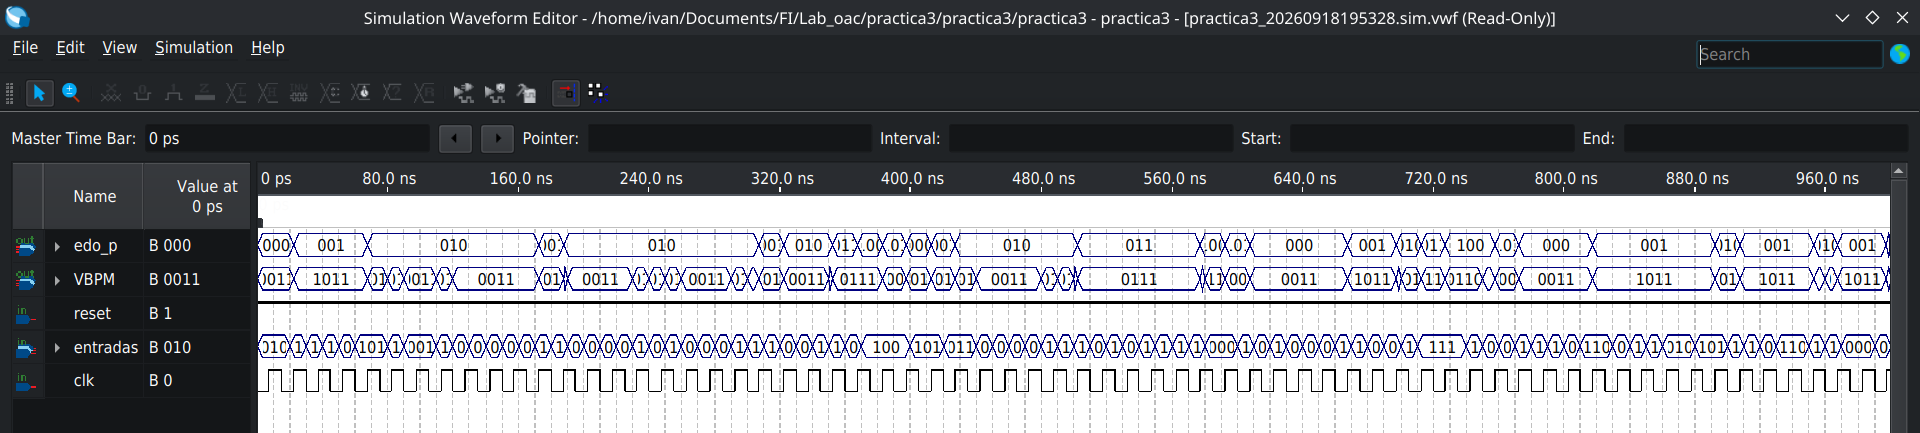
\includegraphics[width=\linewidth]{simulacion_1.png}
  \caption{Primera sección de la simulación. Se mantienen \texttt{reset=1} y combinaciones aleatorias en \texttt{entradas}.}
  \label{fig:simulacion-1}
\end{figure}

La Figura[\ref{fig:simulacion-2}] se muestra el comportamiento anteriormente descrito. En esta gráfica se visualizan los cambios de \texttt{A}, \texttt{B} y \texttt{C} y su relación con los valores de \texttt{edo\_p}. Por ejemplo, cuando la combinación de entradas selecciona una salida condicional que conserva el estado, el valor de \texttt{edo\_p} se repite después del flanco cuando selecciona otra trayectoria,sin embargo aparece la nueva codificación de estado en el siguiente ciclo. Es importante considerar que para las señales de salidas $V$ y $B$ usan lógica positiva, mientras que $P$ y $M$ son activos en bajo, por lo que un cero en estos últimos indica que la función está activa.

\begin{figure}[H]
\centering
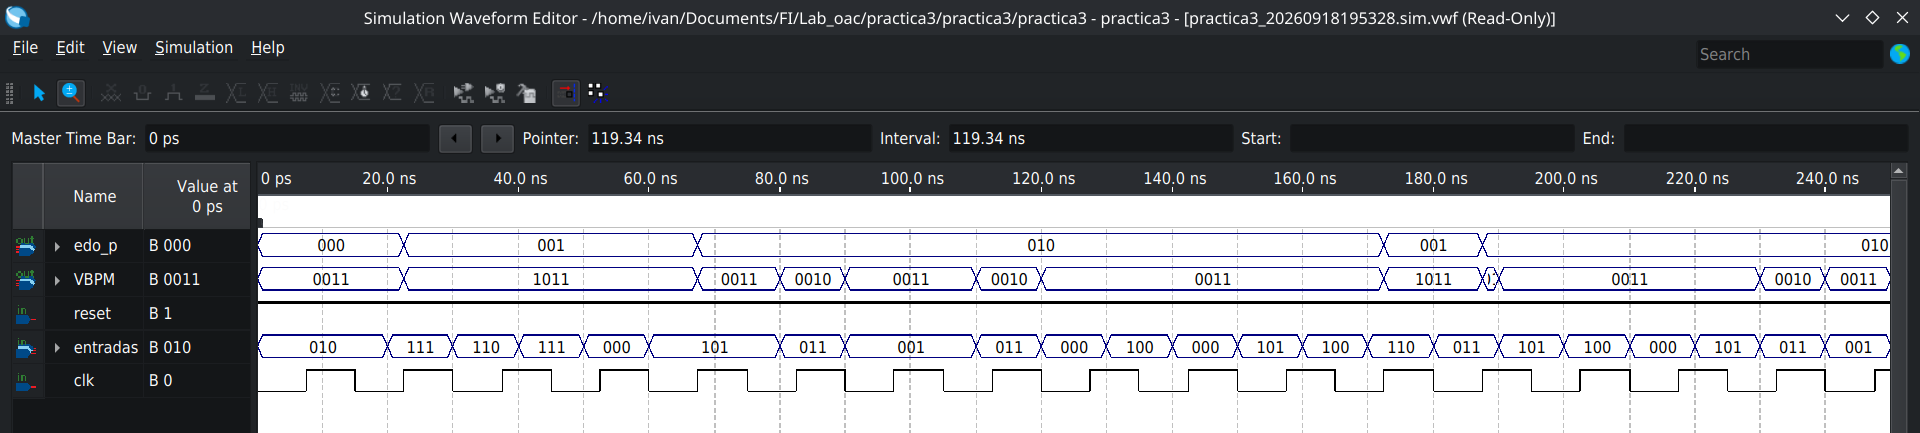
\includegraphics[width=\linewidth]{simulacion_2.png}
\caption{Detalle de la respuesta de \texttt{edo\_p} y \texttt{VBPM} ante cambios aleatorios en las entradas.}
\label{fig:simulacion-2}
\end{figure}

La Figura[\ref{fig:simulacion-3}] corresponde al final de la simulación, donde las entradas se fuerzan a \texttt{111}. Esta condición facilita permite que la carta ASM transicione por todos los estados. La secuencia de \texttt{edo\_p} permite observar el avance por los estados válidos y, al llegar a un estado cuya transición depende de las entradas, la liga almacenada en la ROM determina el siguiente estado. Por lo que  se comprueba el ciclo completo de la máquina y se verifica que el diseño implementado en VHDL cumple con la carta ASM de la lavadora industrial.

\begin{figure}[H]
\centering
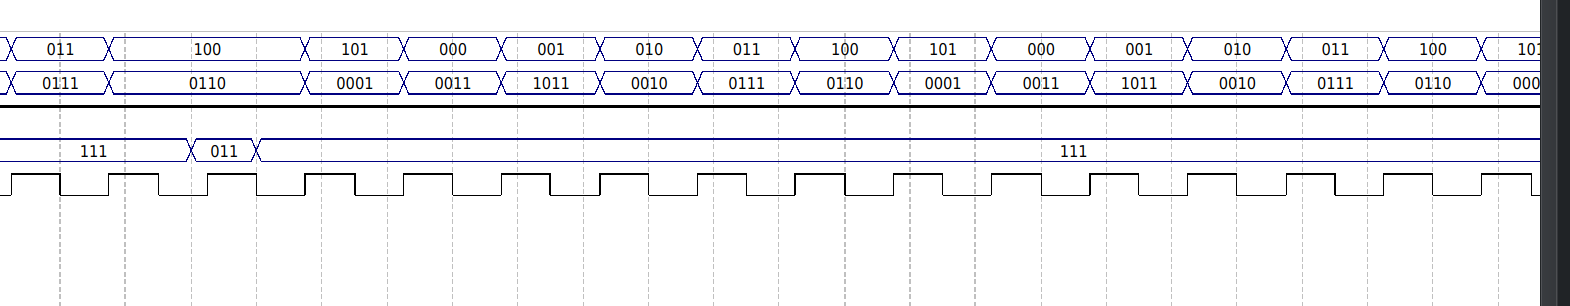
\includegraphics[width=\linewidth]{simulacion_3.png}
\caption{Tramo final forzado con \texttt{entradas=111}; se observa el recorrido completo por los estados de la carta ASM.}
\label{fig:simulacion-3}
\end{figure}

\section{Resultados}

Las Figuras[\ref{fig:bloques-1}] y [\ref{fig:bloques-2}] muestran el diagrama de bloques implementado en Quartus, el cual implementa el flujo de los componentes previamente descritos. Donde el reloj y el botón ingresan al bloque \texttt{clk\_buttom}, el registro entrega el estado presente, el concatenador genera la dirección de seis bits y la ROM produce la palabra de siete bits. El bloque \texttt{div\_datos} distribuye la liga hacia el registro y las salidas \texttt{VBPM} hacia los pines de la tarjeta.

\begin{figure}[H]
\centering
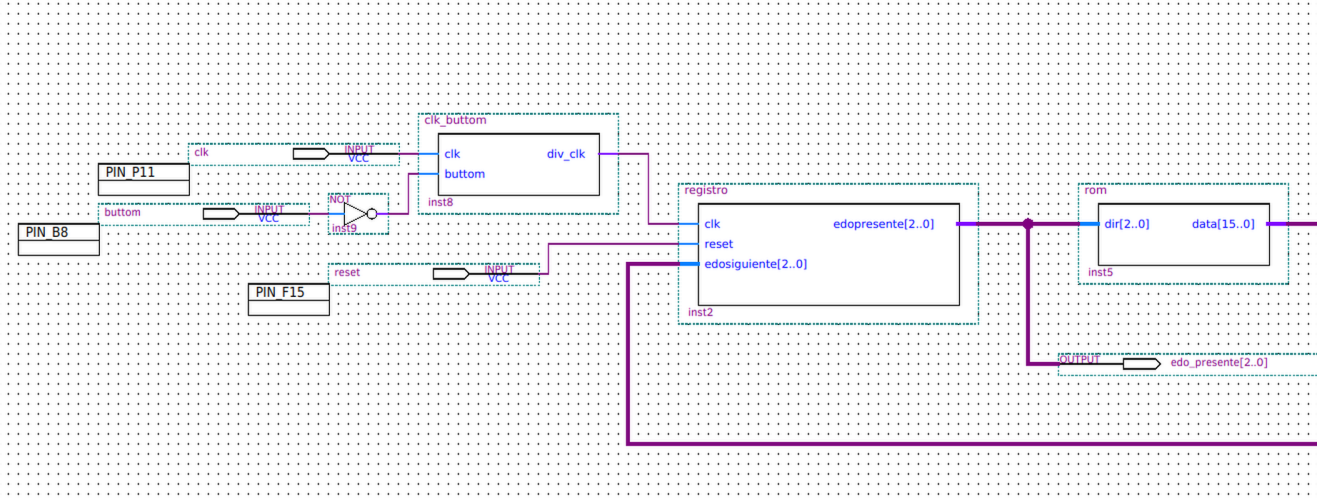
\includegraphics[width=\linewidth]{diagramas_bloques_1.png}
\caption{Interconexión del reloj, el registro de estado, las entradas y el generador de dirección.}
\label{fig:bloques-1}
\end{figure}

\begin{figure}[H]
\centering
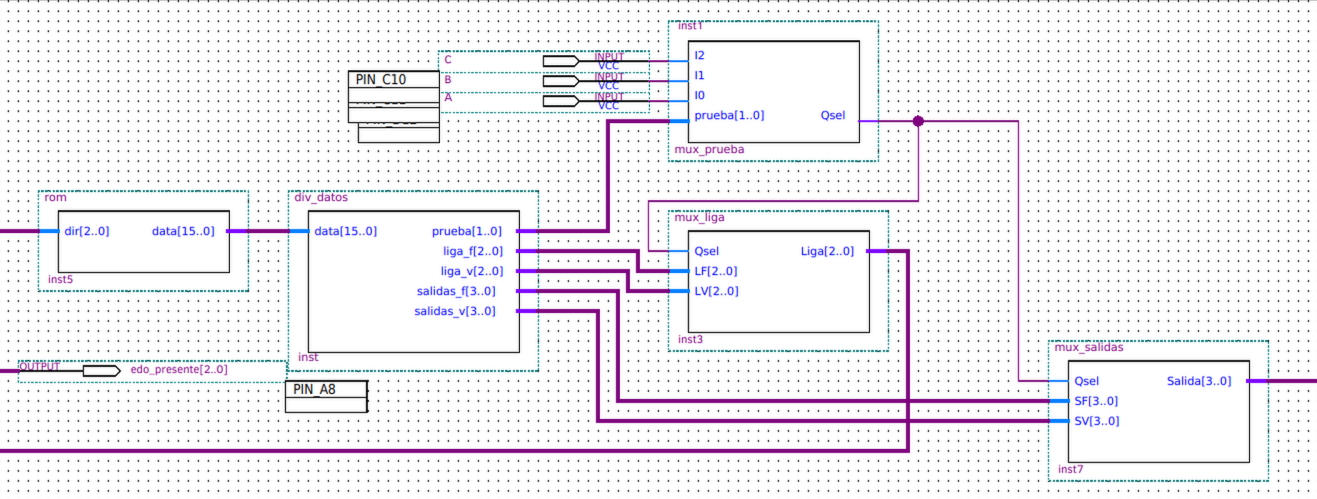
\includegraphics[width=0.92\linewidth]{diagramas_bloques_2.png}
\caption{ROM y división de la palabra de datos en liga y salidas \texttt{VBPM}.}
\label{fig:bloques-2}
\end{figure}

\subsection{Evidencia en la tarjeta FPGA}

Al cargar el diseño en la tarjeta FPGA, se verificó el funcionamiento de la máquina de estados mediante los LEDs asociados al estado presente \texttt{edo\_p} y a las salidas \texttt{VBPM}. Para cada evidencia se seleccionó la combinación de entradas indicada en la tabla de transición y se comparó la respuesta observada con la liga y las salidas almacenadas en la ROM. 

\begin{figure}[H]
\centering
\begin{subfigure}[b]{0.47\linewidth}
  \centering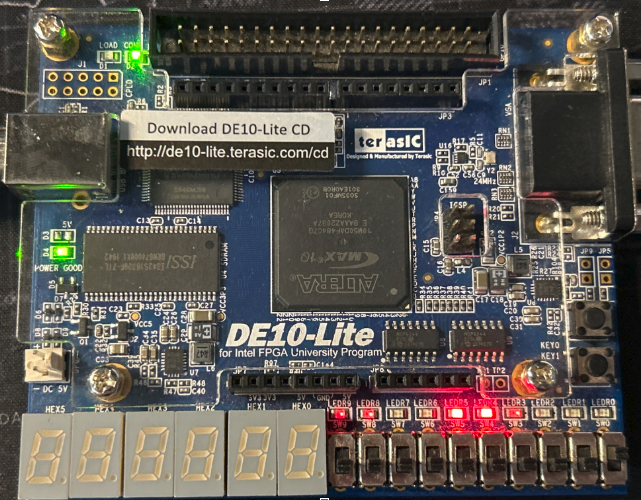
\includegraphics[width=\linewidth]{s0_x0.png}
  \caption{$S_0$, $X=0$: se conserva el estado inicial.}
\end{subfigure}\hfill
\begin{subfigure}[b]{0.47\linewidth}
  \centering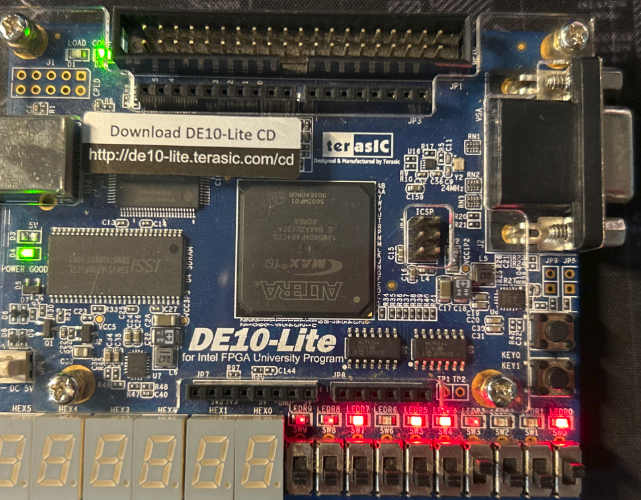
\includegraphics[width=\linewidth]{s0_x1.png}
  \caption{$S_0$, $X=1$: liga hacia $S_1$.}
\end{subfigure}
\caption{Evidencia en tarjeta para las trayectorias del estado $S_0$.}
\label{fig:tarjeta-s0}
\end{figure}

\begin{figure}[H]
\centering
\begin{subfigure}[b]{0.47\linewidth}
  \centering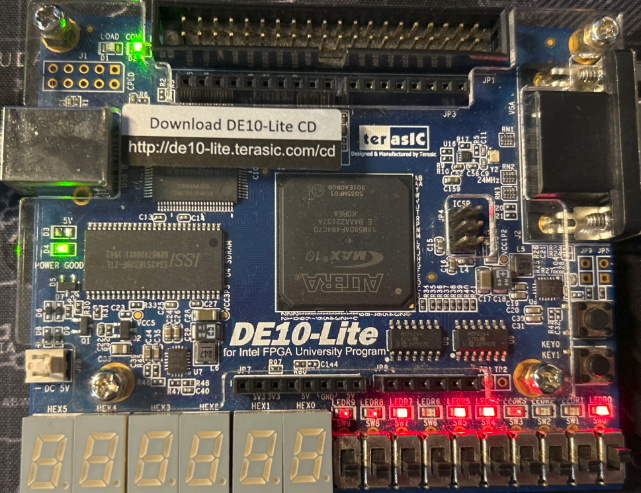
\includegraphics[width=\linewidth]{s1_z0.png}
  \caption{$S_1$, $Z=0$: permanece en llenado.}
\end{subfigure}\hfill
\begin{subfigure}[b]{0.47\linewidth}
  \centering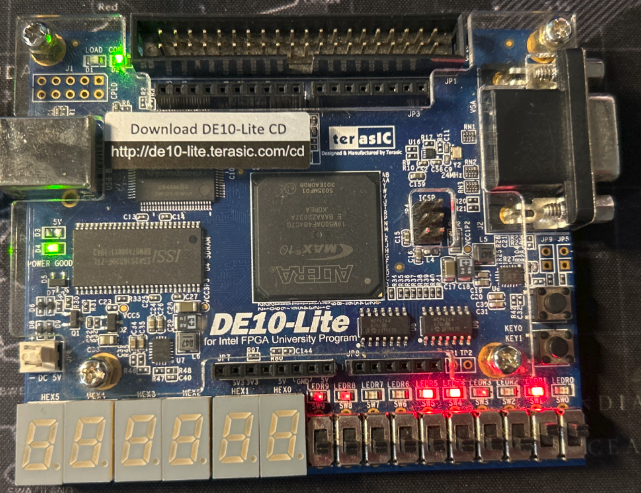
\includegraphics[width=\linewidth]{s1_z1.png}
  \caption{$S_1$, $Z=1$: liga hacia $S_2$.}
\end{subfigure}
\caption{Evidencia en tarjeta para las trayectorias del estado $S_1$.}
\label{fig:tarjeta-s1}
\end{figure}

\begin{figure}[H]
\centering
\begin{subfigure}[b]{0.44\linewidth}
  \centering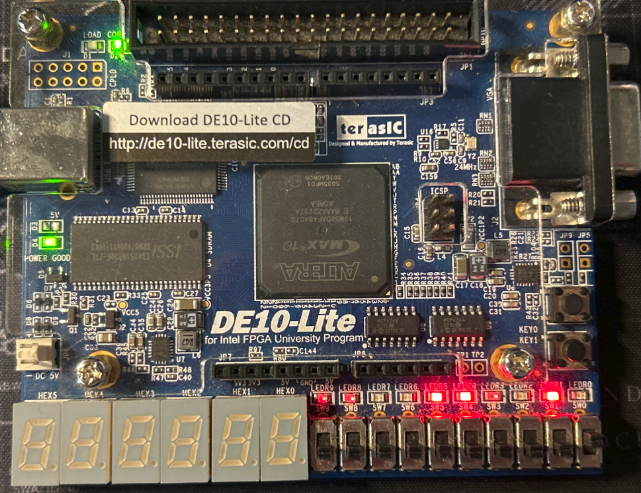
\includegraphics[width=\linewidth]{s2_y0.png}
  \caption{$S_2$, $Y=0$.}
\end{subfigure}\hfill
\begin{subfigure}[b]{0.44\linewidth}
  \centering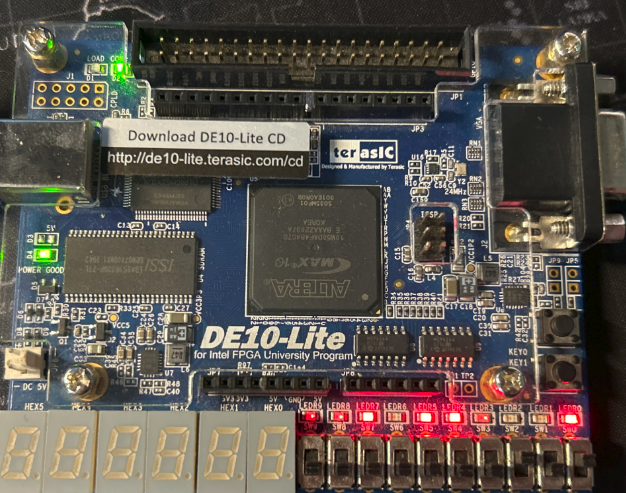
\includegraphics[width=\linewidth]{s2_y1z0.png}
  \caption{$S_2$, $Y=1,Z=0$: liga hacia $S_1$.}
\end{subfigure}\\[3mm]
\begin{subfigure}[b]{0.44\linewidth}
  \centering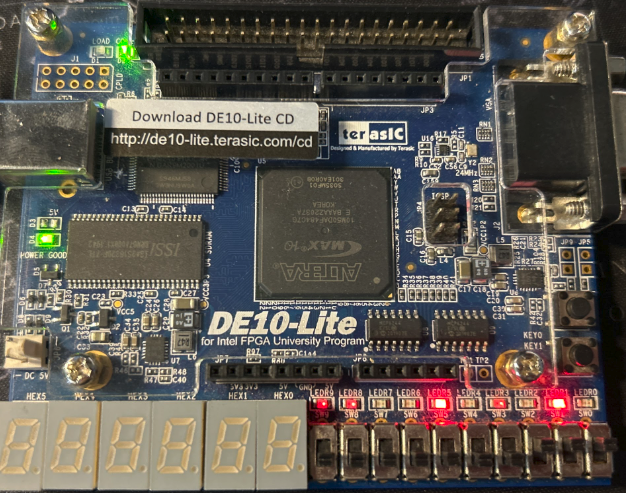
\includegraphics[width=\linewidth]{s2_x0y1z1.png}
  \caption{$S_2$, $X=0,Y=1,Z=1$.}
\end{subfigure}\hfill
\begin{subfigure}[b]{0.44\linewidth}
  \centering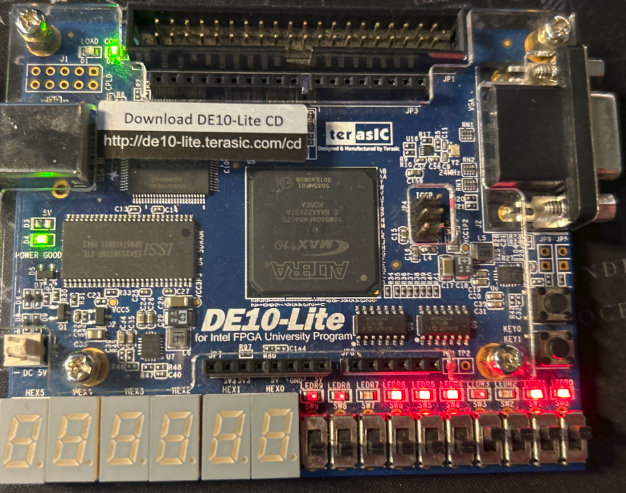
\includegraphics[width=\linewidth]{s2_x1y1z1.png}
  \caption{$S_2$, $X=1,Y=1,Z=1$: liga hacia $S_3$.}
\end{subfigure}
\caption{Evidencia en tarjeta para las cuatro trayectorias del estado $S_2$.}
\label{fig:tarjeta-s2}
\end{figure}

\begin{figure}[H]
\centering
\begin{subfigure}[b]{0.47\linewidth}
  \centering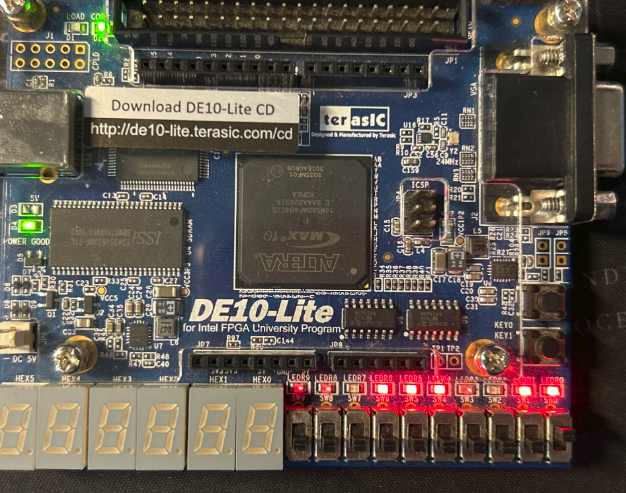
\includegraphics[width=\linewidth]{s3_z0.png}
  \caption{$S_3$, $Z=0$: permanece en drenaje.}
\end{subfigure}\hfill
\begin{subfigure}[b]{0.47\linewidth}
  \centering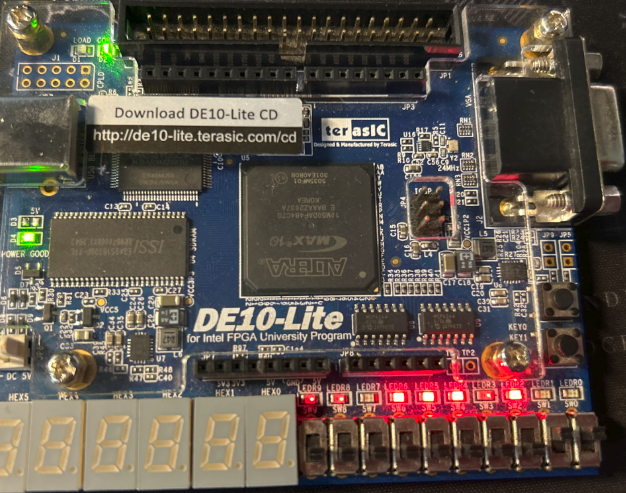
\includegraphics[width=\linewidth]{s3_z1.png}
  \caption{$S_3$, $Z=1$: liga hacia $S_4$.}
\end{subfigure}
\caption{Evidencia en tarjeta para las trayectorias del estado $S_3$.}
\label{fig:tarjeta-s3}
\end{figure}

\begin{figure}[H]
\centering
\begin{subfigure}[b]{0.30\linewidth}
  \centering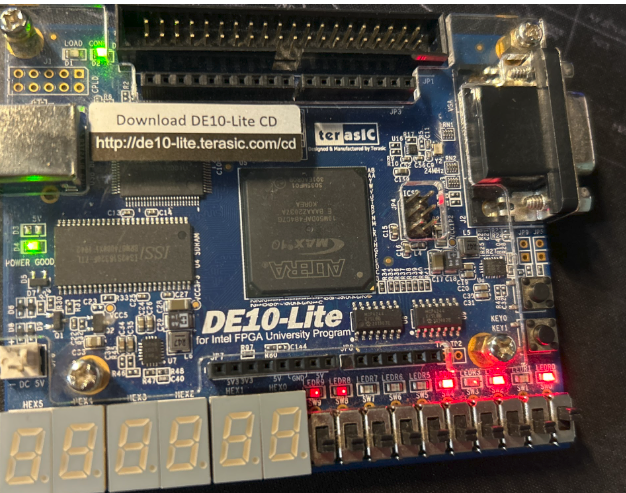
\includegraphics[width=\linewidth]{s4_y0.png}
  \caption{$S_4$, $Y=0$.}
\end{subfigure}\hfill
\begin{subfigure}[b]{0.30\linewidth}
  \centering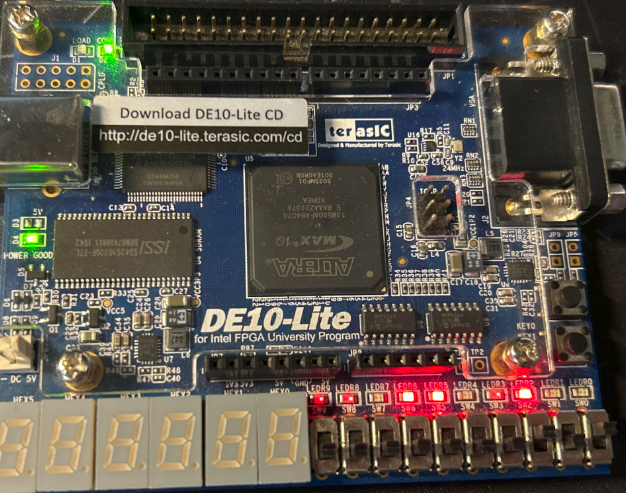
\includegraphics[width=\linewidth]{s4_x0y1.png}
  \caption{$S_4$, $X=0,Y=1$.}
\end{subfigure}\hfill
\begin{subfigure}[b]{0.30\linewidth}
  \centering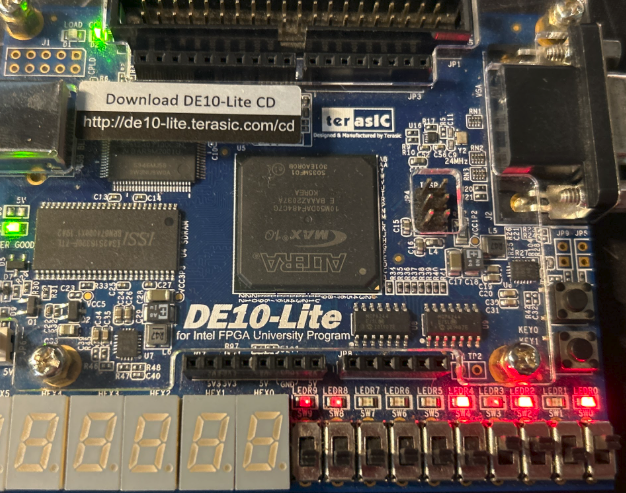
\includegraphics[width=\linewidth]{s4_x1y1.png}
  \caption{$S_4$, $X=1,Y=1$.}
\end{subfigure}
\caption{Evidencia en tarjeta para las trayectorias del estado $S_4$; $Z$ es indiferente en este estado.}
\label{fig:tarjeta-s4}
\end{figure}

\begin{figure}[H]
\centering
\begin{subfigure}[b]{0.47\linewidth}
  \centering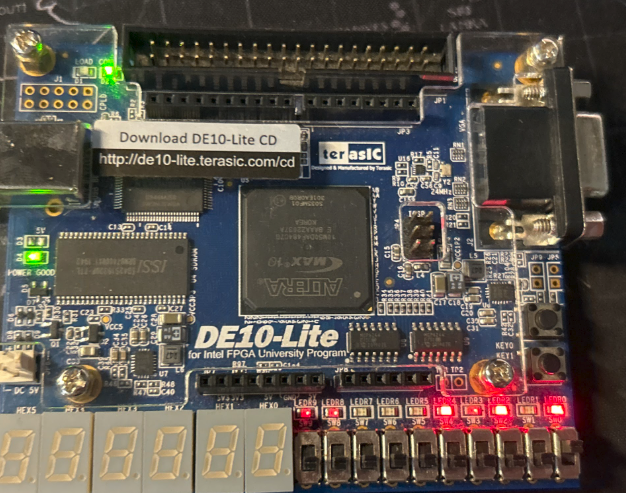
\includegraphics[width=\linewidth]{s5_x0.png}
  \caption{$S_5$, $X=0$: mantiene la alarma.}
\end{subfigure}\hfill
\begin{subfigure}[b]{0.47\linewidth}
  \centering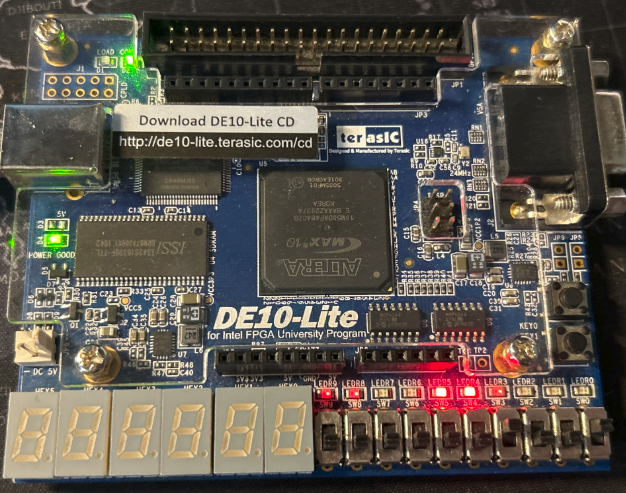
\includegraphics[width=\linewidth]{s5_x1.png}
  \caption{$S_5$, $X=1$: liga hacia $S_0$.}
\end{subfigure}
\caption{Evidencia en tarjeta para las trayectorias del estado $S_5$.}
\label{fig:tarjeta-s5}
\end{figure}

\clearpage
\section{Conclusión}

\paragraph{Percival Ulises Espinoza Matamoros.} Gracias a la realización de la práctica pude comprender la importancia del direccionamiento por trayectoria, ya que al implementar la carta ASM por medio de una memoria ROM junto a otros componentes, donde en la memoria ROM se almacenan las ligas y salidas correspondientes a cada combinación de estado presente y entradas, donde pude observar cómo las entradas determinan la liga y las salidas en cada ciclo de reloj. Al verificar el funcionamiento por medio de la simulación y la implementación física en la tarjeta FPGA, se pudo tener un mejor entendimiento de como funciona el diseño implementado.

\paragraph{Oscar Iván Montiel Juárez.} En esta práctica aplicamos los conceptos vistos en teoría sobre máquinas de estados finitos, cartas ASM, codificación de estados y memorias ROM. Al llevarlos a VHDL y a la tarjeta FPGA, se pudo relacionar la tabla de direccionamiento con el funcionamiento real del circuito, observando cómo las entradas determinan la liga y las salidas en cada ciclo de reloj.

\paragraph{Amy Valentina Veraza García.} El desarrollo mostró la importancia de validar el diseño en más de una etapa. La simulación permitió revisar las transiciones antes de implementarlas, mientras que las pruebas en la tarjeta confirmaron que el registro de estado, la ROM y las salidas responden de acuerdo con la secuencia definida para la llenadora industrial.

\end{document}
